\section{Data}
\label{sec:data}

The given dataset describes multiple channels of EEG data recorded during sleep. There are 14 sleep recordings which are between 490 and 735 minutes long. We are interested in the channels Fp2-F4 and Fp1-F3 as they record activity in the frontal area, where different sleep patterns are shown. [TODO cite something showing this.] The figure~\ref{fig:head_placement} shows where the sensors where placed.

[TODO describe dataset in more detail]

\begin{figure}
	\centering
	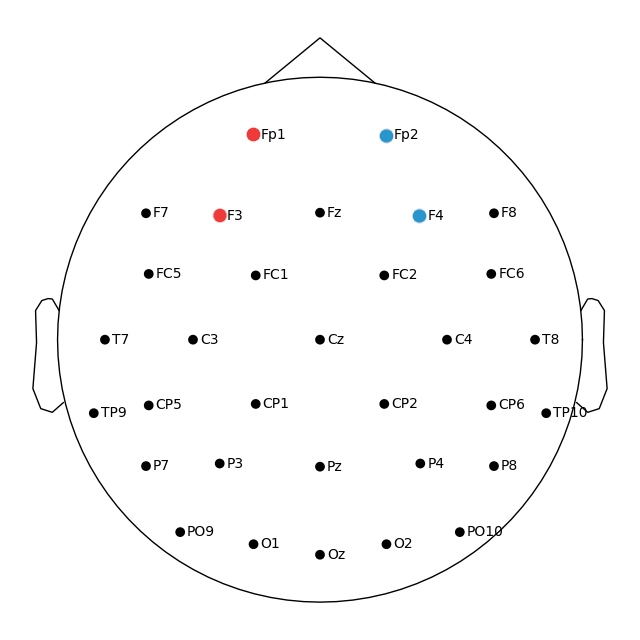
\includegraphics[width=0.7\linewidth]{figs/head_placement}
	\caption{Scheme of sensor placement in recordings of EEG data. Fp1-F3 measure the difference in TODO between Fp1 and F3, both shown in red. Fp2-F4 is analogous for Fp2 and F4, shown in blue. All four points are located in the frontal area.}
	\label{fig:head_placement}
\end{figure}

% length of recordings in minutes: 577, 735, 551, 596, 524, 527, 492, 501, 532, 490, 527, 495, 494, 513

The data was recorded in 512 Hz for channels Fp2-F4 and Fp1-F3. [TODO other channels in other frequencies?] We resample to 200 Hz to reduce data size and standardize all channels.

Very low and very high frequencies often stem from other sources, such as the measurement equipment, breathing or measuring inaccuracies. To get rid of these noises we apply a low pass filter of 30 Hz and a high pass filter of 0.5 Hz.

\section{Algorithm}
\label{sec:algorithm}

We now describe the general structure of the algorithm from reading the data files to the clustering.

First we split the recorded data into 30 second sections. For each of these sections we get the data as a function of amplitude over time. An example segment is shown in the upper figure of~\ref{fig:example_30s_segment}. We apply a Fourier transformation as described in section~\ref{sec:fourier_transformation} and get a function of amplitude over frequency. This gives a frequency based representation of the data. As the sleep stages are characterized by different frequencies and amplitudes, as described in section~\ref{sec:eeg_data_and_sleep_stages}, this will help us distinguishing them. The output of such an FFT can be seen in the lower figure of~\ref{fig:example_30s_segment}. The pseudo code for this processing is 

\begin{algorithm}
	\caption{EEG data processing}\label{alg:process_eeg_data}
	\begin{algorithmic}
		\For{each patient}
		\State Read EEG data from file
		\State Apply a low pass and high pass filter
		\State Resample with frequency 200 Hz
		\State Get one of the channels Fp2-F4, Fp1-F3, C4-A1, F3A2 or C3-A2 (in this order)
		\State Section out the part of data where the patient is asleep
		\For{each 30 second segment of the data}
		\State Do a Fourier transformation (FFT)
		\EndFor
		\State Save all the outputs from the FFT to the patients file
		\EndFor
	\end{algorithmic}
\end{algorithm}


\begin{figure}
	\centering
	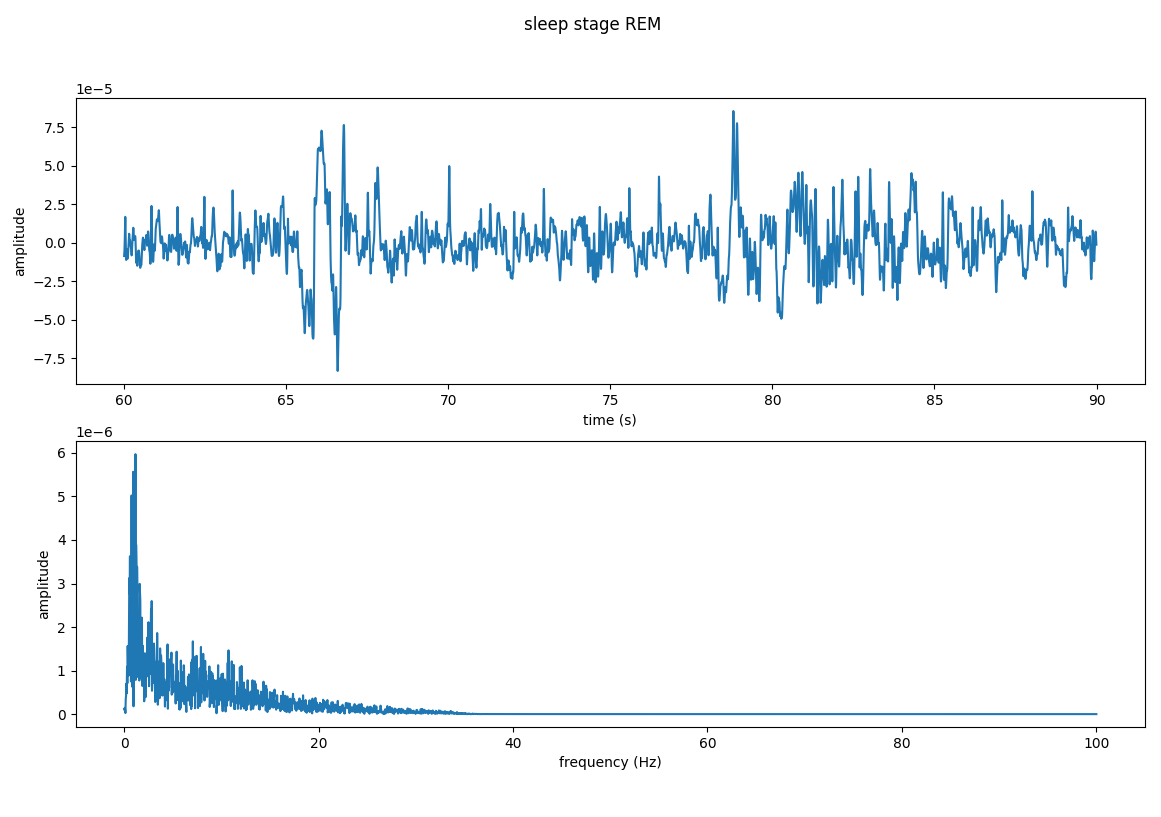
\includegraphics[width=\linewidth]{figs/example_30s_segment}
	\caption{A 30 second segment of the data. The data was filtered with a 0.5 Hz highpass and a 30 Hz lowpass filter. The top shown the recorded signal of the EEG. The bottom shows the output of the Fourier transformation. This segment was assigned the REM sleep stage.}
	\label{fig:example_30s_segment}
\end{figure}


We now have high dimensional data points, as each 30 second segment is represented by the amplitudes for each of the distinct frequencies output by the FFT. Before we can start searching for cluster in the data we want to find a lower dimensional representation. This is were PCA can be used. From the output of algorithm~\ref{alg:pca_of_eeg_data} we get PCs, which reveal the frequencies were the most variance is shown. Under our assumptions this variation is caused by the different sleep stages each recording goes through. We show a visual representation of the data in the first three PC axis in figure~\ref{fig:pca_output_3d}.

\begin{algorithm}
	\caption{Apply PCA to the EEG data}\label{alg:pca_of_eeg_data}
	\begin{algorithmic}
		\For{each patient}
			\State Read FFT output from patients file
			\State Read the sleep stages from another file
		\EndFor
		\State Concatenate FFT data of all patients
		\State Concatenate sleep stages of all patients
		\State Do PCA on the combined FFT data
		\State Transform data according to the PC from the PCA
		\State Visualize the data in the first three axis, with the color corresponding to the sleep stage
	\end{algorithmic}
\end{algorithm}

\begin{figure}
	\centering
	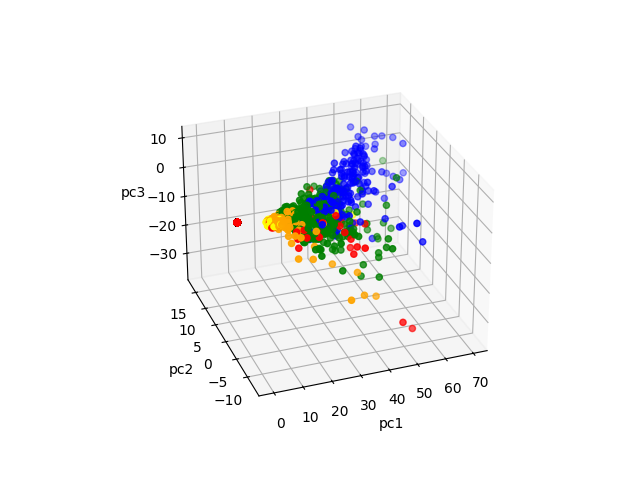
\includegraphics[width=\linewidth]{figs/pca_output_3d}
	\caption{Three dimensional representation of the data. Each 30 second segment is represented by a dot in the color corresponding to the sleep stage this segment is assigned to. Awake is represented by red, orange is REM, yellow is S1, green S2 and blue S3.}
	\label{fig:pca_output_3d}
\end{figure}

If we have a new recording and want to know the sleep stages we have to follow similar steps. First the recording has to be split into 30 second segments. These have to be transformed by a FFT. The output can be converted to the PCA basis by multiplying with the matrix of PCs. Lastly we can get a guess of the sleep stage by using the k nearest neighbor algorithm. The pseudo code is

\begin{algorithm}
	\caption{Get guess for sleep stage}\label{alg:gues_sleep_stage}
	\begin{algorithmic}
		\Require{EEG recording of sleep}
		\For{each 30s segment}
			\State Do FFT on the segment
			\State Multiply FFT output by PCs matrix
			\State Do k nearest neighbor
			\State Save the result of k nearest neighbor
		\EndFor
	\end{algorithmic}
\end{algorithm}
